\documentclass[12pt,a4paper]{article}
\usepackage{multirow}
\usepackage{bm}
\usepackage{AMSFONTS}
\usepackage{amssymb}
\usepackage{latexsym}
\usepackage{graphicx}
\usepackage{subfigure}

\textwidth 6.5in
\textheight 9in
\topmargin 0pt
\linespread{1.5}
\oddsidemargin 0pt
\begin{document}
\title{\huge HW 01 report}
\author{Yilun Zhang\quad Stu ID: 999486337 }
\newtheorem{coro}{\hskip 2em Corollary}[section]
\newtheorem{remark}[coro]{\hskip 2em Remark}
\newtheorem{propo}[coro]{\hskip 2em  Proposition}
\newtheorem{lemma}[coro]{\hskip 2em Lemma}
\newtheorem{theor}[coro]{\hskip 2em Theorem}
\newenvironment{prf}{\noindent { proof:} }{\hfill $\Box$}
\date{1/22/2014}
\maketitle
\section{Basic description}
I applied 3 methods to calculate the mean, standard deviation and the median of Arrival Delay of flights through 1987 to 2012. The first method is use Welford's updating formula to calculate the mean and the standard deviation of Arrival delays. I put the extracted data in the file folder home/data/assignment1. Use for() function to loop over all files use read.csv to get the column of arrival delay. Then also use looping to updating statistic.

The second method is to use shell to get arrival delay column and use frequency table to calculate statistic. I use the FrequencyTable package and add 2 functions to this package, which is to get the s.d. and median.

The Third method is to sample data and estimate the population statistic with the sample mean, s.d., and median.
\section{Results}
The results are saved in result\#.rda files. Because the third method has different results every time I run, there are two result3 file record the results of 2 runs. The results are shown below.\\
\begin{tabular}{lrrr}
\hline\hline
\multicolumn{1}{l}{results}&\multicolumn{1}{c}{}\tabularnewline
\hline
&mean&s.d.&median\tabularnewline
method1&$  6.18538$&31.31200&N/A\tabularnewline
method2&$6.61824$&30.78414&14.00000\tabularnewline
method3-1&$4.187717$&24.841977&0.000000\tabularnewline
method3-2&$4.116142$&25.072014&0.000000\tabularnewline
\hline
\end{tabular}
\section{Summary}
The results of method1 and method2 is very close. I think the result of method2 is more accurate because the first method needs too many steps updating variables to get the result, which accounts for larger error accumulation. The result of method3-1 and method 3-2 is inaccurate. because when doing the sample, I select 100 each file of 1987 to 2007 and 10 files each file of 2008 to 2012, of which the file are separated by month. So the weight of sample of each year is different. I leave the code unchanged because this result also demonstrate that the delay time decreased after 2008 than it is before.

Figure 1 and Figure 2 shows the time of loading file of looping in R and using shell and the time computation takes of methods.
\begin{figure}[!htbp]
\centering
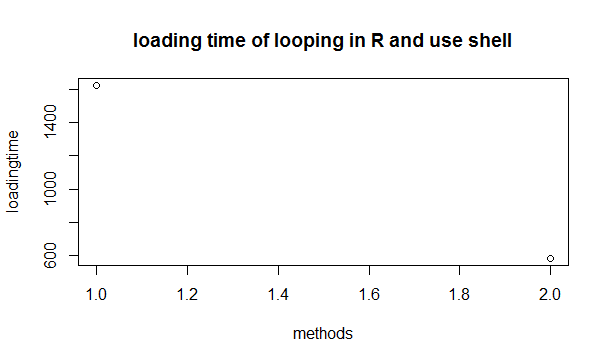
\includegraphics[width=14.5cm]{Rplot.png}
\caption{Figure 1}
\end{figure}
\begin{figure}[!htbp]
\centering
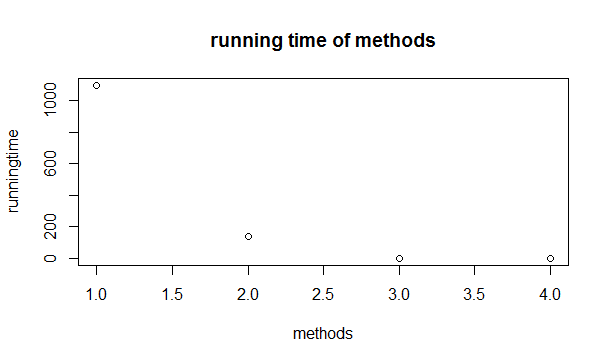
\includegraphics[width=14.5cm]{Rplot1.png}
\caption{Figure 2}
\end{figure}
We can see using shell to extract columns are faster than looping in R, and use frequency table are faster than use  Welford's updating formula. Sampling is a good choice for time saving.

In this assignment I only implement 3 simplest methods. 2 weeks ago I almost know nothing about R and shell. I spent a lot of time learning these. Can you recommend me some books covers material talked in the class, especially on programming on R, so I can catch up with other guys.   



\end{document} 